% Diese Zeile bitte -nicht- aendern.
\documentclass[course=erap]{aspdoc}

%%%%%%%%%%%%%%%%%%%%%%%%%%%%%%%%%
\newcommand{\theGroup}{127}
\newcommand{\theNumber}{A219}
\author{Syrine Aidani \and Adem Trabelsi \and Ahmed Mhamdi}
\date{Wintersemester 2023/2024} 
%%%%%%%%%%%%%%%%%%%%%%%%%%%%%%%%%

\title{Gruppe \theGroup{} -- Abgabe zu Aufgabe \theNumber}

\usepackage{graphicx} 
\usepackage{subcaption}
\graphicspath{{images/}}

\begin{document}
\maketitle

\section{Einleitung}
%TODO: a "Better" image 
%TODO: Mathematical definition of tonwertkorrektur aka. Section 2.1 GRA_0219.pdf 
Der Schwerpunkt dieses Projekts liegt auf der Konvertierung farbiger Bilder in Graustufen und der darauf folgenden Durchführung einer Tonwertkorrektur. 
Als Eingabe lesen wir zuerst 24bpp PPM (P6) Pixelbilder. Jeder Farbpixel wird als Vektor mit den drei Farbkanälen Rot R, Grün G und Blau B definiert. Durch die Berechnung eines gewichteten Durchschnitts D, wandeln wir zunächst die Bilder in Graustufen um. Die entstandenen Graustufenbilder unterziehen wir dem Tonwertkorrektur mittels eine Interpolationsfunktion, die ermöglicht eine reibungslose Anpassung der Graustufenwerte zwischen den nutzerspezifizierte Stützpunkten. 
Zuletzt erstellen wir eine neue Datei im 8bpp PGM (P5) Format und dort hineinschreiben wir die berechneten Werte nach dem Tonwertkorrektur.

%Image file
  \begin{figure}[h]
    \begin{subfigure}{0.5\linewidth}
      \centering
      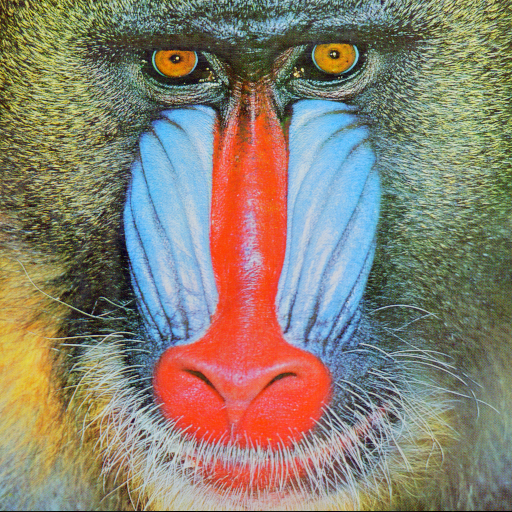
\includegraphics[width=\linewidth]{mandrill-2}
      \caption{EingabeBild}
      \label{fig:eingabe}
    \end{subfigure}%
    \begin{subfigure}{0.5\linewidth}
      \centering
      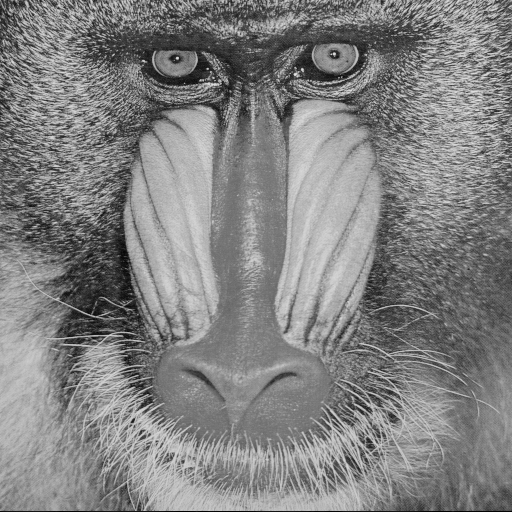
\includegraphics[width=\linewidth]{mandrillausgabe-2}
      \caption{AusgabeBild}
      \label{fig:ausgabe}
    \end{subfigure}
  \end{figure}


Die Abbildungen \ref{fig:eingabe} und \ref{fig:ausgabe} repräsentieren ein Eingabebild und das entsprechende Ergebnis unserer Hauptimplementierung unter Verwendung der Standardwerte für Schwarz-, Weiß- und Mittelwerte für die Tonwertkorrektur.


Im Folgenden werden wir die ausgewählten Ansätze diskutieren, auf ihre Korrektheit prüfen und ihre Performanz analysieren.


\section{Lösungsansatz}


\subsection{Graustufen Konvertierung}
%TODO mention SIMD implementation
%TODO BIBTEX for literature aka. \cite[text]{keylist} ->not final yet 
\subsubsection{Intuitiver Ansatz: Durchschnitt}

Die folgende Umrechnungsformel ist der Durchschnitt der RGB Komponenten:
 \[ D = \frac{R + G + B}{3}  \]
Die Durchschnittsmethode ist ebenfalls problematisch, da sie jedem Komponenten den gleichen Gewicht zuweist.

\subsubsection{Grün-Kanal Ansatz}
Das menschliche Auge ist am empfindlichsten gegen Grün, daher ist die Verwendung von Grün eine schnellere , aber ungenauere  Alternative zur Umwandlung von RGB in Luminanz.
\[D = G\] 

\subsubsection{Luminanz Ansatz}
Die Luminanz $Y$ dient als Maß für die Helligkeit von Bildpunkten, entsprechend der Wahrnehmung durch das menschliche Auge. Da das Auge besonders empfindlich für die Farbe Grün ist und weniger empfindlich für Blau, wird eine Gewichtung der RGB-Komponenten benötigt, um die Farbwahrnehmung des menschlichen Auges zu berücksichtigen. [1]
In unserem Kontext, bei der Arbeit mit einem PPM-Bild, das der ITU-R-Empfehlung BT.709 entspricht [2], wird die folgende Umrechnungsformel gemäß Rec. 709 für die Berechnung der CIE-Luminanz aus den linearen RGB-Komponenten verwendet:
 \[Y = 0.2125R + 0.7154G + 0.0721B \] [3]
Die ITU-R Empfehlung BT.709 definiert auch das gamma-codierte Luma $Y'$, die eine gewichtete Summe der nichtlinearen (nach Gamma-Korrektur) RGB-Komponenten entspricht, wobei gilt:
 \[Y' = 0.2126R' + 0.7152G' + 0.0722B' \] [4]
Die Verwendung der Luminanz bietet eine genauere Darstellung der tatsächlichen Helligkeit und eignet sich daher besser für die 8-Bit-Kodierung von Graustufen. Man muss jedoch das Bild zuvor in einen linearen RGB-Farbraum umwandeln, um den gewichteten Durchschnitt auf die linearen RGB-Komponenten anwenden zu können.
Alternativ kann jede der drei Farbkomponenten auf das berechnete Luma Y' gesetzt werden. Dies ermöglicht eine einfachere Berechnung und ist in der Praxis oft ausreichend für Graustufenbilder.
 \[ D = Y' = 0.2126R' + 0.7152G' + 0.0722B' \]   



\subsection{Tonwertkorrektur}

\subsubsection{Lineare Interpoltion}
%TODO Define lineare interpolation 
%TODO Implementation + SIMD
%TODO mention bilinear interpolation: Better alternative for stable contast and brightness values 
%TODO Question 5: diff between lineare and quadratic: No ovrflow vs. Overflow - Overflow's impact on resulting images. --> Next how we implement quadratic and how we dealt with the overflow problem. 

\subsubsection{Quadratische Interpolation}
%TODO Define quadratic interpolation 
\paragraph{Gauß-Jordan}
%TODO Description: Trivial approach: solve the system using Gauß-Jordan Algorithmus. Note: our system is always solvable 
%TODO: Proof solvability of the system (PROOF SUBSECTION) 
%TODO: Rounding errors -> Pivoting  (Why Pivoting avoids Rounding errors in a nutshell)
%TODO: Argumentation: Choice of float 
%TODO: Conclusion-> Overkill solution to our problem BUT this solution is mathematically the closest to the described scheme -> Use in accuracy testing 

\paragraph{Lagrange Interpolation}
%TODO: Description: Lagrange interpolation -> Bad for computation -> Modified Lagrange 
%TODO: Proof: From lagrange to modified version of lagrange 
%TODO: Problem: Unstability 
%TODO: Conclusion: -> Newton interpolation
\paragraph{Newton Interpolation}
%TODO: Description: Newton interpolation

\subsection{Hauptimplementierung}
%TODO: Description: Hauptimplementierung (Best alternative: Quadratic Interpolation Newton + Grayscale: Luminanaz Ansatz) + SIMD Opt.
%TODO: Mention vergleichsimplemetierung: 1) Trivial for accuracy testing 
%TODO                                    2) Hauptimpl - SIMD for performance analysis


\section{Korrektheit}
%TODO: Approach: One to one translation of Testing 
\subsection{Genauigkeit}
\subsection{Korrektheit}

\section{Performanzanalyse}
%TODO: Mention environment
\subsection{Quadratic Interpolations-Algorithmen}
%TODO Gauß, Lagrange, Blagrange, Newton

\subsection{SIMD Optimierungen}
%TODO Grayscale Newton + LUT 
%TODO LUT not that performant -> Better alternative for ARM- Architecture
\subsection{Hauptimplementierung}
%TODO Hauptimplemtierung vs trivial

\section{Zusammenfassung und Ausblick}
%TODO Zusammenfassung
%TODO Cubic interpolation (4th, 5th ...)
%TODO Horner's method 
%TODO better alternatives: accecpt overflow -> mem|time opt (uint8_t instead of floats) or to predict overflow (lower and higher bound) -> Convenience
%TODO more opt: Multithreading

% TODO: Fuegen Sie Ihre Quellen der Datei Ausarbeitung.bib hinzu
% Referenzieren Sie diese dann mit \cite{}.
% Beispiel: CR2 ist ein Register der x86-Architektur~\cite{intel2017man}.
\bibliographystyle{plain}
\bibliography{Ausarbeitung}{}

\end{document}